\documentclass[main]{subfiles}

\begin{document}

\begin{figure}[!ht]
  \centering
  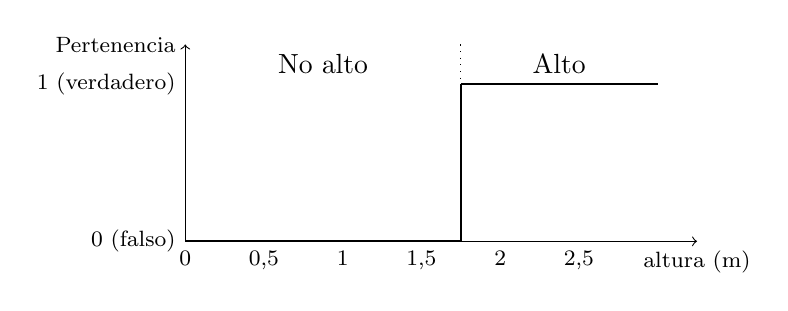
\begin{tikzpicture}

    % horizontal axis
    \draw[->] (0,0) -- (6.5,0) node[anchor=north] {\footnotesize altura (m)};
    % labels
    \draw	(0,0) node[anchor=north] {\footnotesize 0}
    		(1,0) node[anchor=north] {\footnotesize 0,5}
    		(2,0) node[anchor=north] {\footnotesize 1}
    		(3,0) node[anchor=north] {\footnotesize 1,5}
    		(4,0) node[anchor=north] {\footnotesize 2}
    		(5,0) node[anchor=north] {\footnotesize 2,5};

    % vertical axis
    \draw[->] (0,0) -- (0,2.5) node[anchor=east] {\footnotesize Pertenencia};
    % labels
    \draw	(0,0) node[anchor=east] {\footnotesize 0 (falso)}
    		(0,2) node[anchor=east] {\footnotesize 1 (verdadero)};

    % funcion
    \draw[thick] (0,0)--(3.5,0);
    \draw[thick] (3.5,0)--(3.5,2);
    \draw[thick] (3.5,2)--(6,2);
    \draw[dotted] (3.5,2.5)--(3.5,0);
    \draw (4.75,2.25) node {Alto}; %label
    \draw (1.75,2.25) node {No alto}; %label

  \end{tikzpicture}

  \caption{Representación de la pertenencia de los elementos para la lógica clásica. \label{fig:altoclasica}}
\end{figure}

\end{document}
